\documentclass{article}
\usepackage{graphicx}
\usepackage{amsmath}



\begin{document}
\section{LATR Optical Design}

The large aperture receiver is composed of an a array of 85 three lens cameras in an hexagonal packing. Each camera is made of three plano convex silicon lenses and a Lyot stop which reimages the primary mirror. A silica prism (with one side perpendicular to the camera axis and the other side at an angle) is placed in front of the first lens to keep the camera axes parallel. The silica prism surface tilt and clocking is defined such that the chief ray of the center field of each camera lands at the center of the detector focal plane. 


The hexagonal packaging of the optics tubes is described by the equation \begin{equation}
\begin{bmatrix}x \\ y\end{bmatrix} = \frac{d_{\rm center}}{\sqrt{3}} \begin{bmatrix} \sqrt{3} & \sqrt{3}/2 \\ 0 & 3/2 \end{bmatrix} \begin{bmatrix}q \\ r\end{bmatrix},
\end{equation} where $d_{\rm center}$ is the center to center distance between optics tubes ($219 \rm mm$) and the parameter $q$ and $r$ are indexing integers between -5 and 5. The field lens in the camera is a $20~\rm cm$ diameter lens while the second and third lenses are limited to be $17~\rm cm$ in diameter to allow for clamping clearance. 

\paragraph{TMA}

For the TMA design, the surface of each lens $z(r)$ is defined as a conic surface of revolution plus 8 polynomial terms in $r$, with $r$ measured from the center of the lens according to the equation\begin{equation}
	z(r) = \frac{cr^2}{1+\sqrt{1-(1+k)c^2r^2}} + \sum_{j=1}^{8} \alpha_{2j} r^{2j}, 
\end{equation}
where $c$ is the curvature (defined as $c=1/R$, with R the radius of curvature), $k$ is the conic constant, and $\alpha_{2j}$ are the even coefficients of the polynomial expansion. 



\begin{figure}

	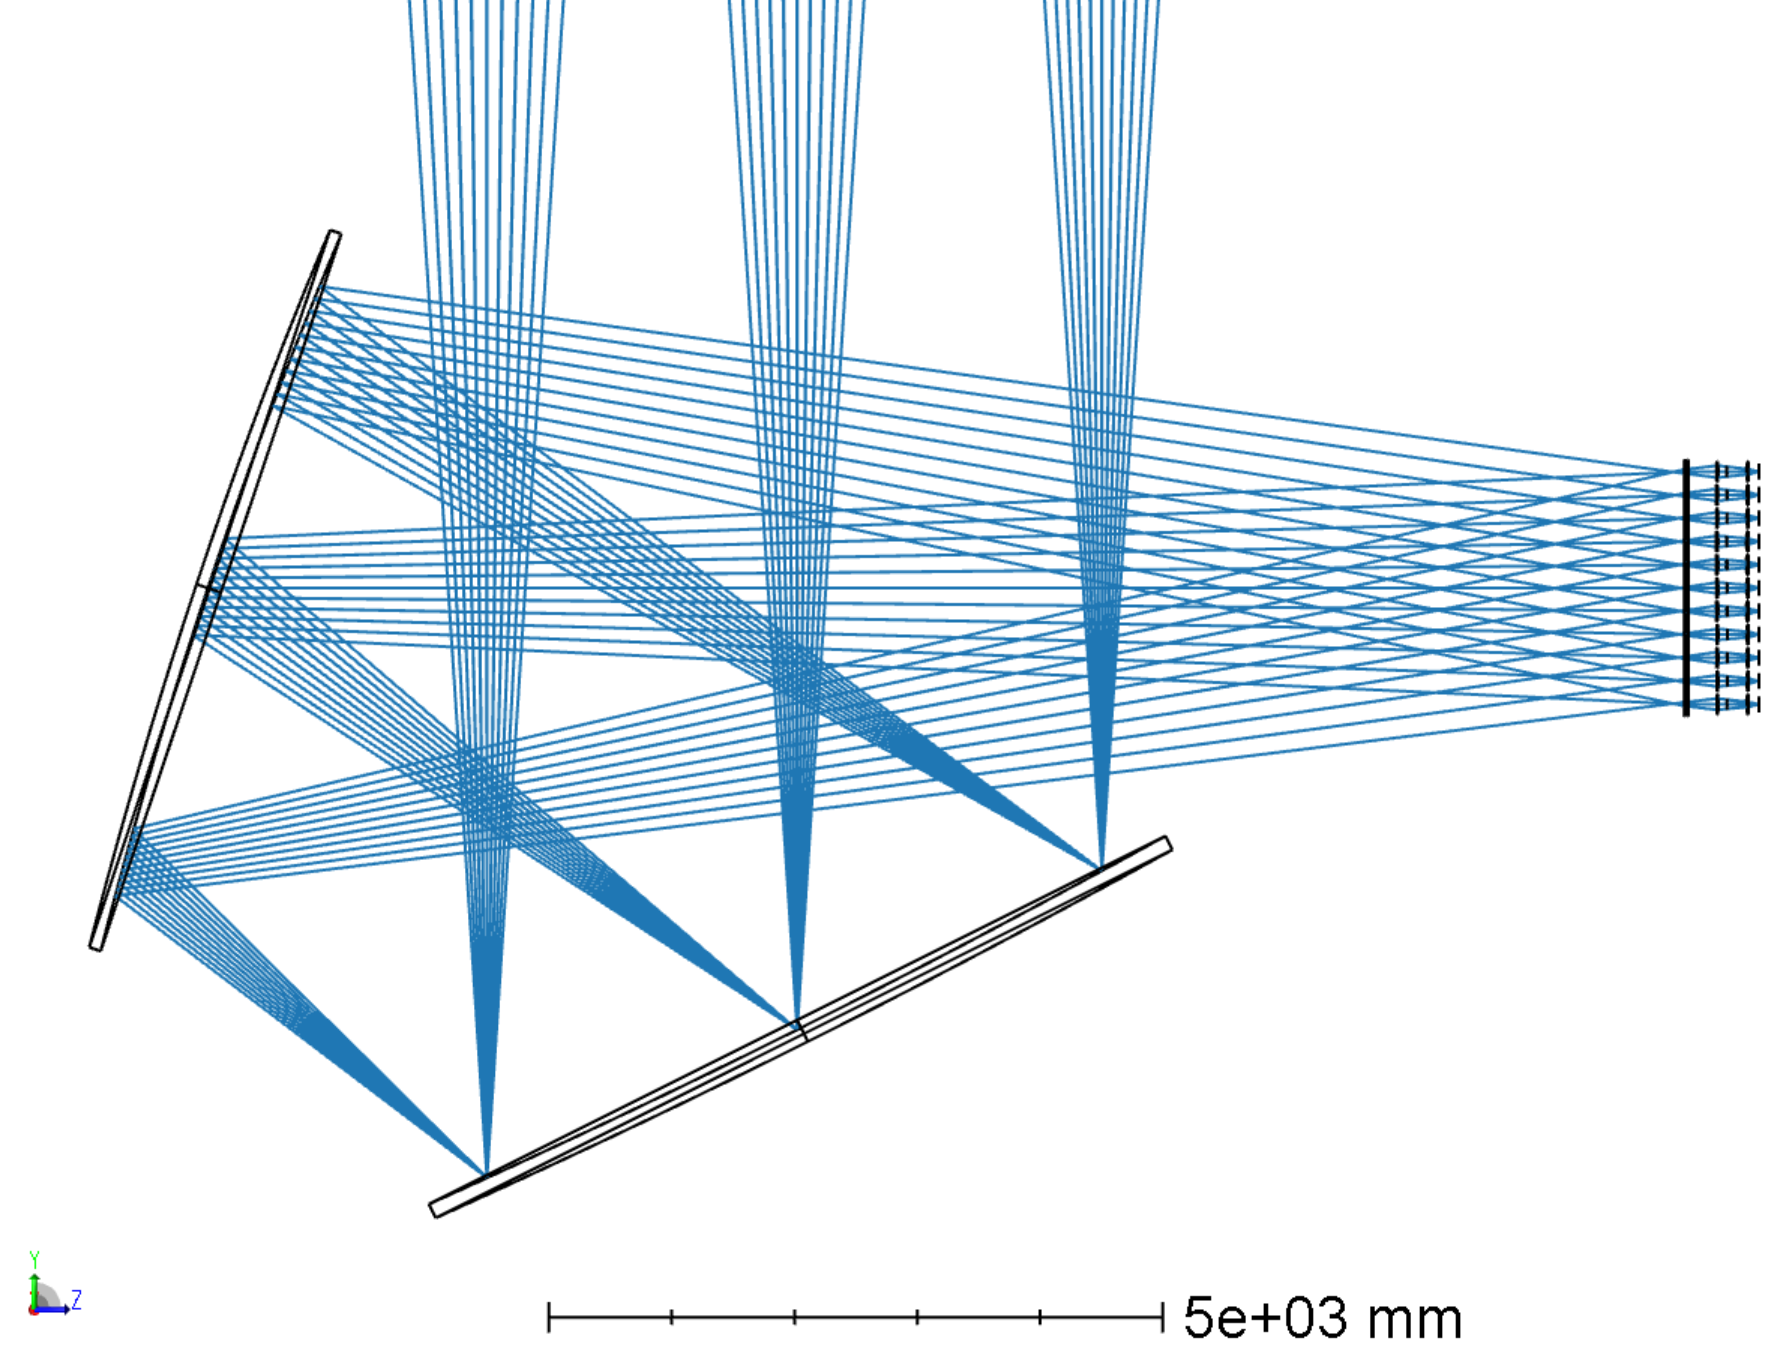
\includegraphics[width=0.48\textwidth]{CD_3DLayout.png}
	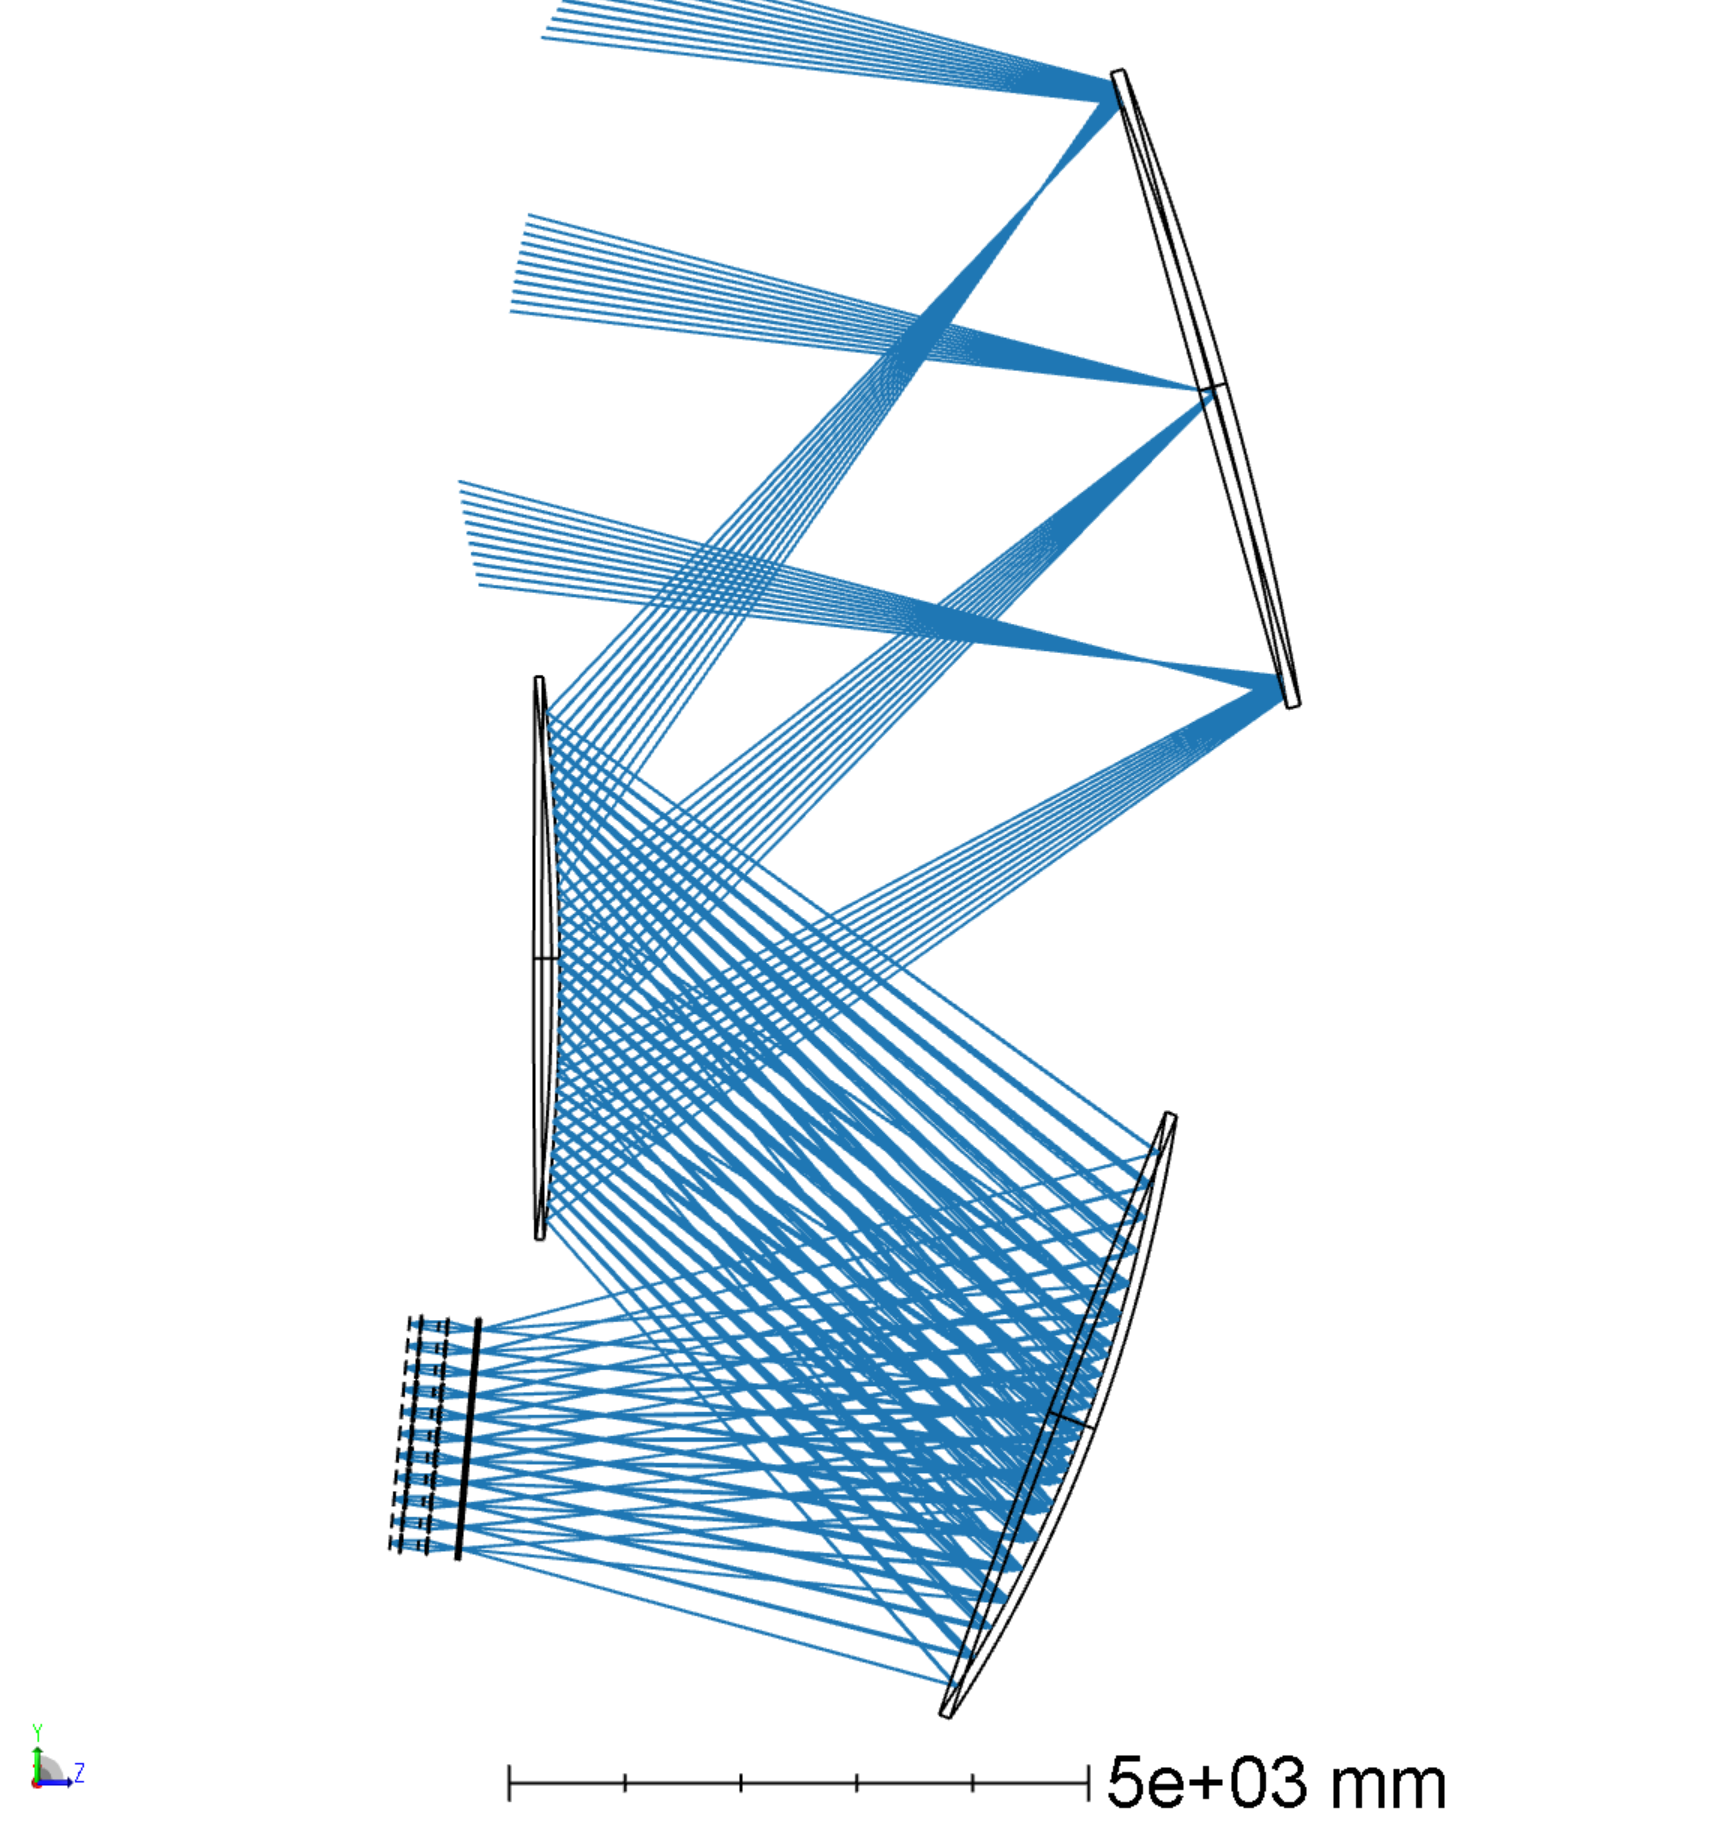
\includegraphics[width=0.48\textwidth]{TMP_3DLayout.png}
	
	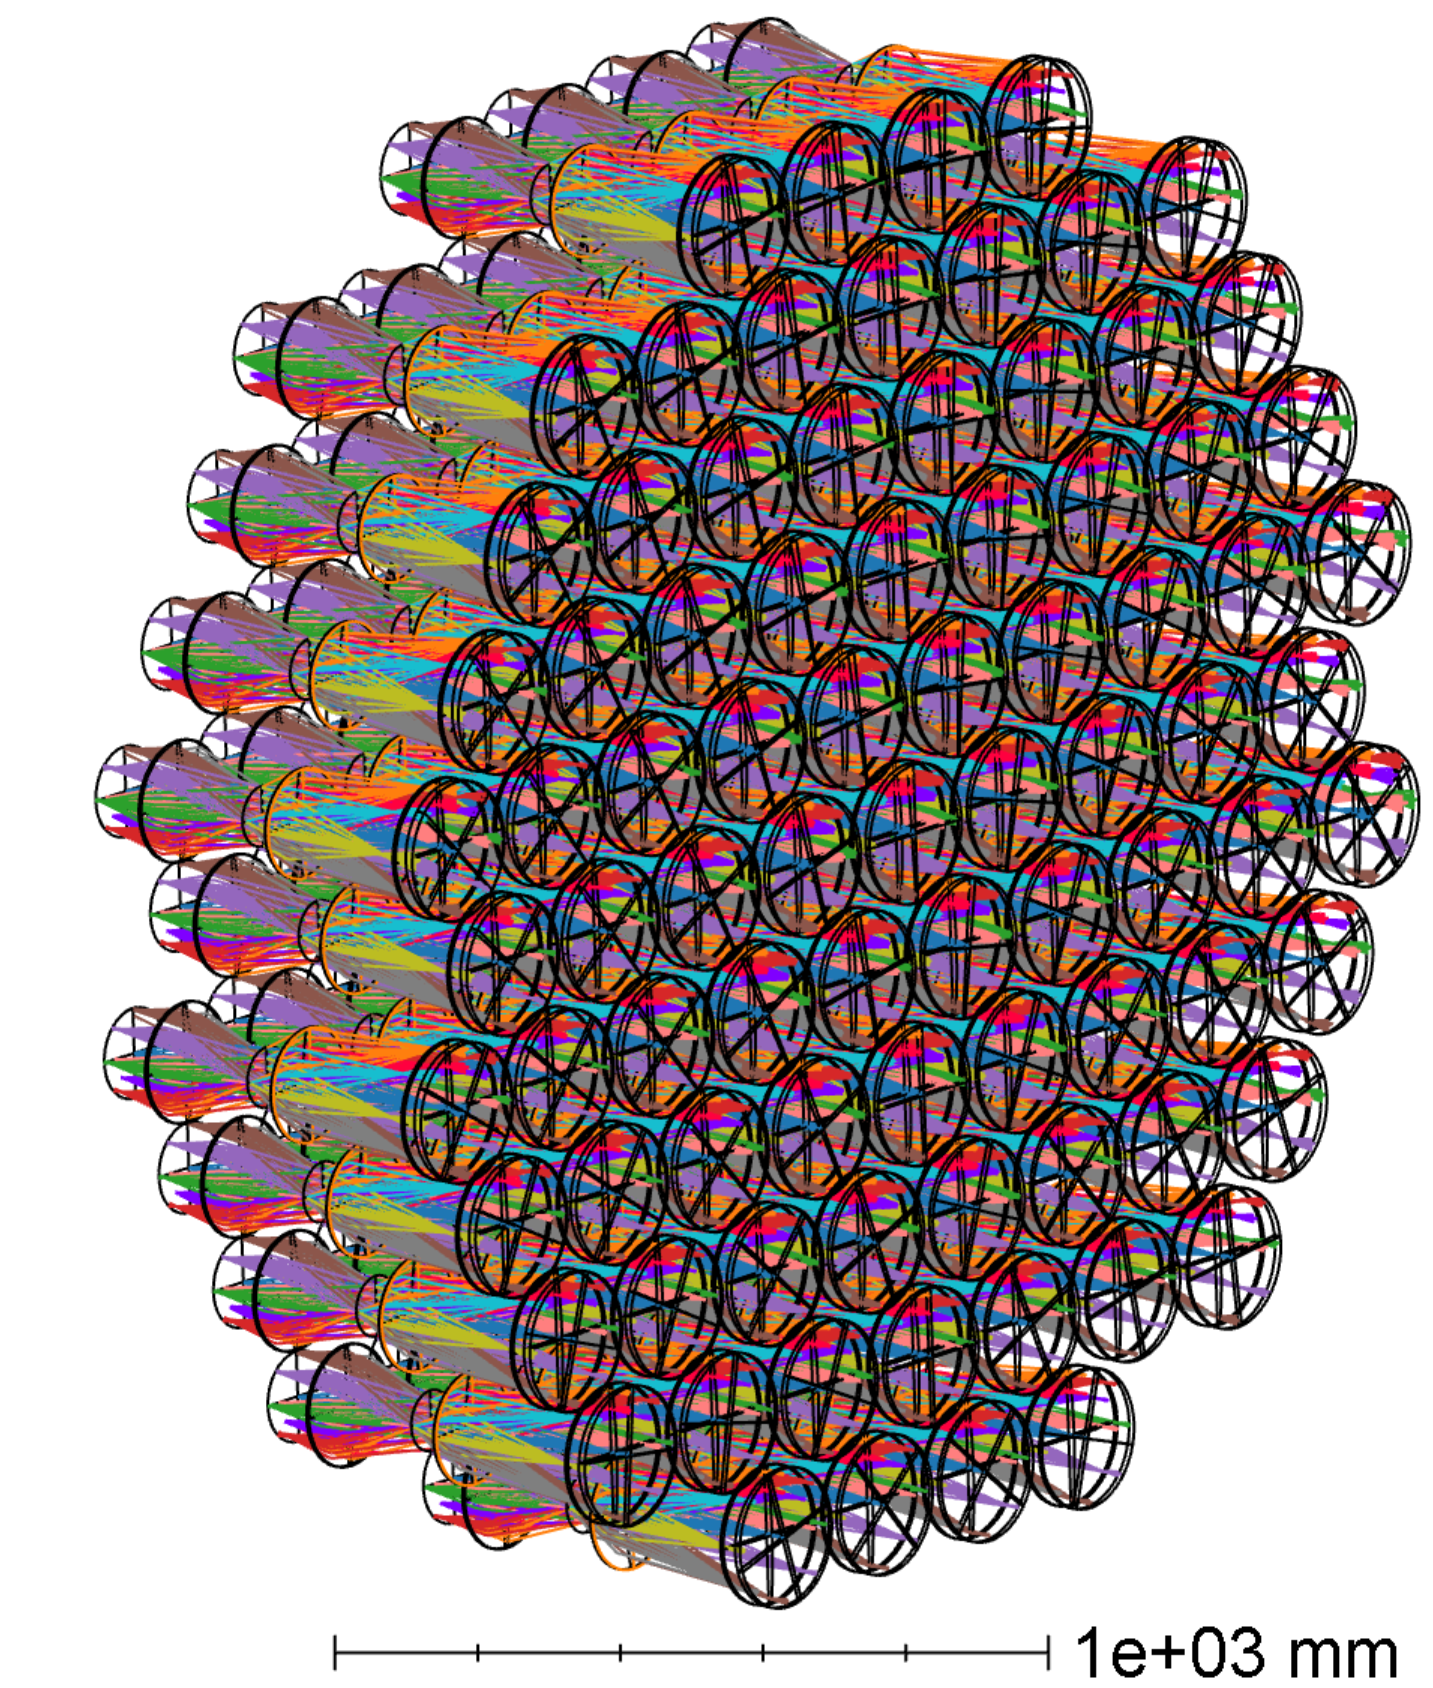
\includegraphics[width=0.48\textwidth]{TMP_cams.PNG}
	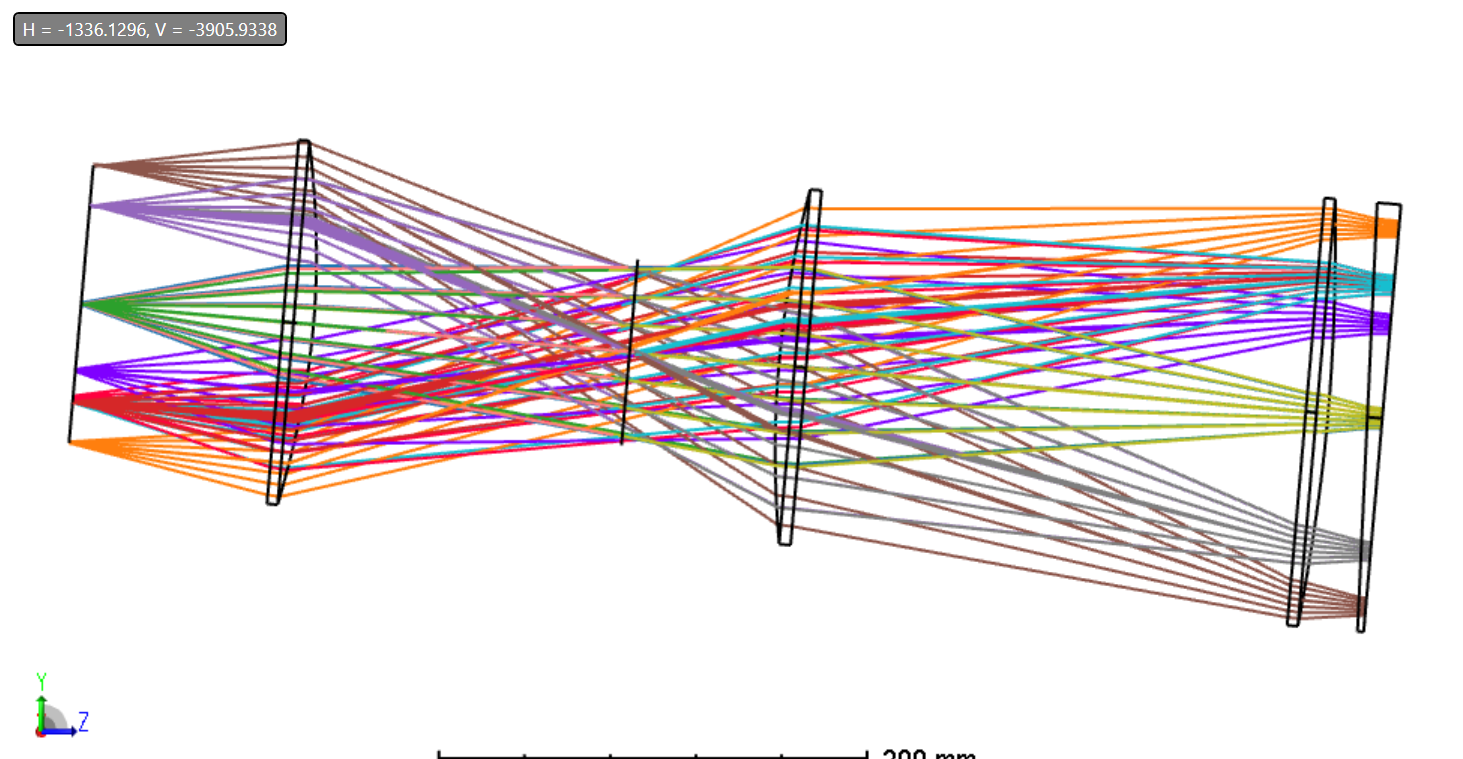
\includegraphics[width=0.48\textwidth]{TMP_cam1_layout.PNG}	
	
	\caption{Raytrace of the large aperture telescope configurations. Sideview of the 85 camera system on the Crossed Dragone (top left) and TMA (top right).}
	\label{fig:opticsDesign}
\end{figure}

\paragraph{Crossed Dragone} The crossed Dragone camera lenses are composed of biconic lenses whith \begin{equation}
	z_{biconic} = \frac{c_x x^2 + c_y y^2}{1+ \sqrt{1-(1-k_x)c_x^2 x^2-(1+k_y)c_y^2y^2}} + \sum_{i=1}^{16} \alpha_i x^i + \sum_{j=1}^{16} \beta_j y^j 
\end{equation}

with curvatures given by  $c_x=\frac{1}{R_x}$ and $c_y=\frac{1}{R_y}$ and conic constants $k_{x,y}$




\end{document}
